%% Basierend auf einer TeXnicCenter-Vorlage von Mark M�ller
%%%%%%%%%%%%%%%%%%%%%%%%%%%%%%%%%%%%%%%%%%%%%%%%%%%%%%%%%%%%%%%%%%%%%%%

% W�hlen Sie die Optionen aus, indem Sie % vor der Option entfernen  
% Dokumentation des KOMA-Script-Packets: scrguide

%%%%%%%%%%%%%%%%%%%%%%%%%%%%%%%%%%%%%%%%%%%%%%%%%%%%%%%%%%%%%%%%%%%%%%%
%% Optionen zum Layout des Artikels                                  %%
%%%%%%%%%%%%%%%%%%%%%%%%%%%%%%%%%%%%%%%%%%%%%%%%%%%%%%%%%%%%%%%%%%%%%%%

\documentclass[%
a4paper,							% alle weiteren Papierformat einstellbar
%landscape,						% Querformat
10pt,								% Schriftgr��e (12pt, 11pt (Standard))
%BCOR1cm,							% Bindekorrektur, bspw. 1 cm
%DIVcalc,							% f�hrt die Satzspiegelberechnung neu aus
%											  s. scrguide 2.4
twoside,							% Doppelseiten
%twocolumn,						% zweispaltiger Satz
%halfparskip*,				% Absatzformatierung s. scrguide 3.1
%headsepline,					% Trennline zum Seitenkopf	
%footsepline,					% Trennline zum Seitenfu�
%titlepage,						% Titelei auf eigener Seite
%normalheadings,			% �berschriften etwas kleiner (smallheadings)
%idxtotoc,						% Index im Inhaltsverzeichnis
%liststotoc,					% Abb.- und Tab.verzeichnis im Inhalt
%bibtotoc,						% Literaturverzeichnis im Inhalt
%abstracton,					% �berschrift �ber der Zusammenfassung an	
%leqno,   						% Nummerierung von Gleichungen links
%fleqn,								% Ausgabe von Gleichungen linksb�ndig
%draft								% �berlangen Zeilen in Ausgabe gekennzeichnet
]
{book}

%\pagestyle{empty}		% keine Kopf und Fu�zeile (k. Seitenzahl)
%\pagestyle{headings}	% lebender Kolumnentitel  

%% Packungen %%%%%%%%%%%%%%%%%%%%%%
%% Deutsche Anpassungen %%%%%%%%%%%%%%%%%%%%%%%%%%%%%%%%%%%%%
\usepackage[czech]{babel}
\usepackage[T1]{fontenc}
\usepackage{xcolor}
\usepackage{lmodern} %Type1-Schriftart f�r nicht-englische Texte


%% Packages f�r Grafiken & Abbildungen %%%%%%%%%%%%%%%%%%%%%%
\usepackage{graphicx} %%Zum Laden von Grafiken
%\usepackage{subfig} %%Teilabbildungen in einer Abbildung
%\usepackage{pst-all} %%PSTricks - nicht verwendbar mit pdfLaTeX

%% Beachten Sie:
%% Die Einbindung einer Grafik erfolgt mit \includegraphics{Dateiname}
%% bzw. �ber den Dialog im Einf�gen-Men�.
%% 
%% Im Modus "LaTeX => PDF" k�nnen Sie u.a. folgende Grafikformate verwenden:
%%   .jpg  .png  .pdf  .mps
%% 
%% In den Modi "LaTeX => DVI", "LaTeX => PS" und "LaTeX => PS => PDF"
%% k�nnen Sie u.a. folgende Grafikformate verwenden:
%%   .eps  .ps  .bmp  .pict  .pntg
\babelprovide[import,main]{czech}

%% Bibliographiestil %%%%%%%%%%%%%%%%%%%%%%%%%%%%%%%%%%%%%%%%%%%%%%%%%%
%\usepackage{natbib}

\begin{document}

\pagestyle{empty} %%Keine Kopf-/Fusszeilen auf den ersten Seiten.


%%%%%%%%%%%%%%%%%%%%%%%%%%%%%%%%%%%%%%%%%%%%%%%%%%%%%%%%%%%%%%%%%%%%%%%
%% Ihr Artikel                                                       %%
%%%%%%%%%%%%%%%%%%%%%%%%%%%%%%%%%%%%%%%%%%%%%%%%%%%%%%%%%%%%%%%%%%%%%%%

%% eigene Titelseitengestaltung %%%%%%%%%%%%%%%%%%%%%%%%%%%%%%%%%%%%%%%    
%\begin{titlepage}
%Einsetzen der TXC Vorlage "Deckblatt" m�glich
%\end{titlepage}

%% Angaben zur Standardformatierung des Titels %%%%%%%%%%%%%%%%%%%%%%%%
%\titlehead{Titelkopf }
%\subject{Typisierung}
\title{Basics of LaTEX}
\author{AK}
%\and{Der Name des Co-Autoren}
%\thanks{Fu�note}			% entspr. \footnote im Flie�text
%\date{}							% falls anderes, als das aktuelle gew�nscht
%\publishers{Herausgeber}

%% Widmungsseite %%%%%%%%%%%%%%%%%%%%%%%%%%%%%%%%%%%%%%%%%%%%%%%%%%%%%%
%\dedication{Widmung}

\maketitle 						% Titelei wird erzeugt

%% Zusammenfassung nach Titel, vor Inhaltsverzeichnis %%%%%%%%%%%%%%%%%
%\begin{abstract}
% F�r eine kurze Zusammenfassung des folgenden Artikels.
% F�r die �berschrift s. \documentclass[abstracton].
%\end{abstract}

%% Erzeugung von Verzeichnissen %%%%%%%%%%%%%%%%%%%%%%%%%%%%%%%%%%%%%%%
\tableofcontents			% Inhaltsverzeichnis
%\listoftables				% Tabellenverzeichnis
%\listoffigures				% Abbildungsverzeichnis


%% Der Text %%%%%%%%%%%%%%%%%%%%%%%%%%%%%%%%%%%%%%%%%%%%%%%%%%%%%%%%%%%

\part{Basics}
\chapter{Installation}
\section{Einführung}
LaTeX selbst ist keine Applikation wie MS Worls aber es ist ein \textbf{Softwarepacket} für die Textverarbeitung. Ein Benutzer arbeitet nur mit Textdateien. Die Formatierung führ man durch den Kommands. Um eine Literaturform zu erhalten, muss der Text kompilliert werden. Deswegen gibt es keine Applikation mit dem Namen LaTeX aber man kann über LaTex wie über eine Programmiersprache nachdenken. Es gibt die Applikationen wie z.B. MikTeX die einen Latex und einen Kompiler dafür enthalten. MikTeX selbs hat aber nicht gute GUI, deswegen muss man noch einen GUI wie z.B. TeXnicCenter installieren. Andere Möglichkeit für Windows ist TexMaker, der Latex, Kompiler und auch GUI enthält. 

Um MiKtex zu installieren empfehlt man zuerst die specifischen Build y.b. von einer Uniresität herunterzuladen und dann es aus diesem Datei installieren. Es ist gut (auf Tschechisch) beschereibt in:
https://latex.fekt.vut.cz/instalace-miktex-a-spol-pc-windows/instalace-miktex/

Konfiguration von PDF Viewer in TeXnicCe
\chapter{Writing standards}
čšřý

Česká republika
Definiton of text parameters is done with help of commands. Commands are defined with \textbackslash after which the name of command follows \textcolor {blue}{\bf\textbackslash commandAK\bf}. There is no space between "'\textbackslash"'and name of command. After that often often follows parameters in curly brackets = braces. Some commands have more parameters in more curly brackets, some have one curly bracket and some parameters in square brackets. 

La
\chapter{Textaufteilen}
Längeren Texte wie Bücher oder längeren Artikel ist besser wenn man es in mehrere Dateien gibt. In jeder Datei kann zum Beispiel eine Kapitel geschrieben sein.
Includes enable to include other "`.tex"' files.
\section{Creating Includes}
\normalsize$C(T_i)$

\chapter{Equations}

$C(T_i)$
\[
C(T_i) = L_i \cdot n_i
\]
where:
\\$C(T_i)$ - Total isolated communication cost of task $T_i$ 
\\$L_i$ - Communication load of one hop of task $T_i$
\\$n_i$ - Number of hops from task $T_i$ to destination

\[
C(T_i) = L_i \cdot n_i + \sum_{k=1}^{j} L_j \cdot n_j
\]
\\where:
\\$C(T_i)$ - Total communication cost of task $T_i$ 
\\$L_i$ - Communication load of one hop of task $T_i$
\\$n_i$ - Number of hops from task $T_i$ to destination
\\$L_j$ - Communication load of one hop of task $T_j$
\\$n_j$ - Number of common hops for task $T_j$ and $T_i$
\chapter{Errors}
\subsection{Pdf Viewer Compilation Error in TeXnicCenter}
Auf die Karte Build → Define Output Profiles klicken. Im neuen Fenster auf Latex→PDF klicken und dann auf die Karte Viewer. Statt \textit{acroview} wie Server zu haben, muss man \textit{acroviewAnn} schreiben. Dabei ist \textit{nn} ein Versionsjahr von Acrobat. Z.B. 2024 → nn=24 Konfiguration von PDF Viewer in TeXnicCenter ist nötig.  

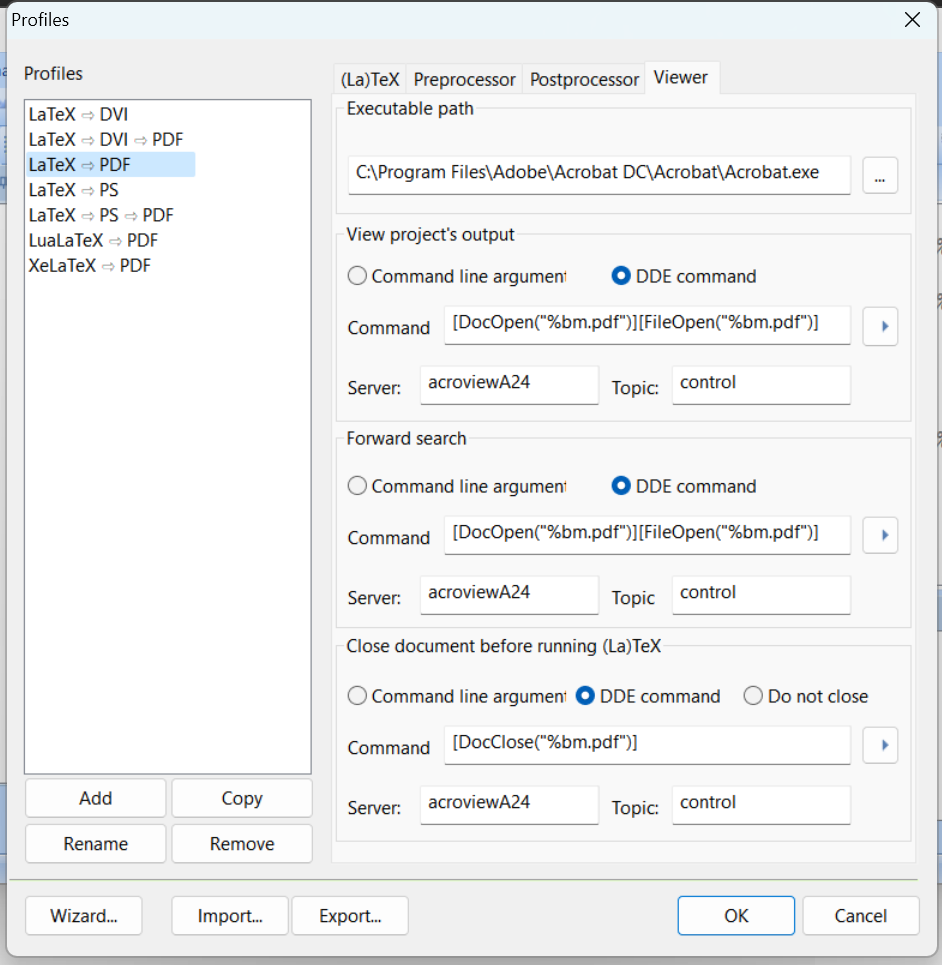
\includegraphics[width=\linewidth]{LTX_Sources/texniccenter-pdf-config.png}
\end{document}
